\documentclass{beamer}
\usetheme[
  block=fill,
  background=dark,
  titleformat=smallcaps,
  progressbar=frametitle,
  numbering=none,
]{metropolis}

% Math
\usepackage{amsmath}
\usepackage{amssymb}
\usepackage{stmaryrd}

% Code listing
\usepackage{minted}
\usemintedstyle{monokai}
%\usemintedstyle{native}
%\usemintedstyle{tango}
\newcommand{\icode}[1]{\mintinline{haskell}{#1}}

% Graphics
\usepackage{graphics}
\usepackage{pdfpages}
\graphicspath{{figures/}} % Location of the graphics files

\newcommand\todo[1]{\textcolor{red}{#1}}

% Box macro
\newcommand{\ex}[2]{
  \vfill
  \begin{alertblock}{#1}
    #2
  \end{alertblock}
}
%----------------------------------------------------------------------------

% Beamer
\title{AlgoRhythm}
\subtitle{A Library for Algorithmic Music Composition}
\author{Joris ten Tusscher, Cas van der Rest, Orestis Melkonian}
\date{April 5, 2018}
\institute{Universiteit Utrecht}

\begin{document}
	\maketitle

  \begin{frame}{Some definitions}
    	\begin{itemize}
    	\item
        \textbf{Melody}: Notes played in \emph{sequence}
        \item
        \textbf{Chords/harmony}: Notes played \emph{simultaneously}
        \item
        \textbf{Scale}: a sequence of ascending notes, beginning and starting on the same note.
    	\end{itemize}

       	i.e: C major = C, D, E, F, G, A, B, C

        Or in intervals: 2, 2, 1, 2, 2, 2, 1
    \end{frame}

    \begin{frame}{Some definitions}
    	A piece of music is said to be in a \textbf{key} if it (primarily) uses notes from a certain scale

        \textbf{Diatonic} music is music that uses scales that have the same pattern as we saw before (2,2,1,2,2,2,1).
    \end{frame}

    \begin{frame}[fragile=singleslide]{Music DSL: Representation}
	Basically, you want to know when to make noise and when to remain silent.

    Two pieces of music can be composed in parallel or sequentially.
    \begin{minted}[baselinestretch=1, fontsize=\small, autogobble]{haskell}
type Duration = Rational

data Music a = Music a :+: Music a
             | Music a :=: Music a
             | Note Duration a
             | Rest Duration
    \end{minted}
	\end{frame}

    \begin{frame}[fragile=singleslide]{Music DSL: Representation}
    In order to provide export functionalities, we use a \icode{MusicCore} type and a typeclass \icode{ToMusicCore}.
    \begin{minted}[baselinestretch=1, fontsize=\small, autogobble]{haskell}
type PitchClass = C | Cs | D ... As | B
type Octave = Oct0 | Oct1 ... Oct5 | Oct6
type PitchAttribute = Dynamic Dynamic
                    | Articulation Articulation

type MusicCore =
  Music ((PitchClass, Octave), [PitchAttribute])
    \end{minted}

    This ensures that all the necessary information is there when exporting a piece of music
	\end{frame}
    \begin{frame}[fragile=singleslide]{Music DSL: Representation}
    (Abstract) scales and chords are represented as intervals between notes, i.e:

    \icode{major = [P1,M2,M3,P4,P5,M6,M7] -- Major scale}
    \icode{d7b5 = [P1, M3, A4, Mi7] -- Half diminished chord}

    There are many constants for various scales and chords (, as well as common durations:

    \begin{minted}[baselinestretch=1, fontsize=\small, autogobble]{haskell}
qn = 1%4
    \end{minted}
	\end{frame}

    \begin{frame}[fragile=singleslide]{Music DSL: Manipulation}
	Music can be constructed and manipulated using various operators

    \begin{minted}[baselinestretch=1, fontsize=\small, autogobble]{haskell}
 -- quarter note C in the 4th octave, played softly
 let n = (C#4 <: [PPP]) <| qn

 -- A half note rest
 let r = (hn~~)

 -- Instantiate an abstract chord
 let cMaj7 = ((C =| maj7) <#) 3 <|| wn
    \end{minted}
	\end{frame}

    \begin{frame}[fragile=singleslide]{Music DSL: Manipulation}
	A melody in our DSL:

    \begin{minted}[baselinestretch=1, fontsize=\small, autogobble]{haskell}
 line [ (C#6 <: [Dynamic PP]) <| wn
      , (D#6 <: [Dynamic MP]) <| wn
      , (hn~~)
      , (C#6 <: [Dynamic F_]) <| qn
      , (D#6 <: [Dynamic F_]) <| qn
      , (C#6 <: [Dynamic F_]) <| qn
      , (B#5 <: [Dynamic F_]) <| qn
      , (D#6 <: [Dynamic MF]) <| qn
      , (C#6 <: [Dynamic MP]) <| wn
      , (F#5 <: [Dynamic P ]) <| wn
      ]
    \end{minted}
	\end{frame}

    \begin{frame}[fragile=singleslide]{Music DSL: Manipulation}
	There's also some operators for common operations:

    \begin{minted}[baselinestretch=1, fontsize=\small, autogobble]{haskell}
 -- Transposition
 C ~> M3 == E

 -- Retrograded (mirroring)
 let music' = (music><)

 -- Time scaling
 let music' = music *~ (1%5)

    \end{minted}

	Also, \icode{Music} is a functor!

	\begin{minted}[baselinestretch=1, fontsize=\small, autogobble]{haskell}
	let rhythm = const () <$> music
    \end{minted}
	\end{frame}

	{\usebackgroundtemplate{%
  	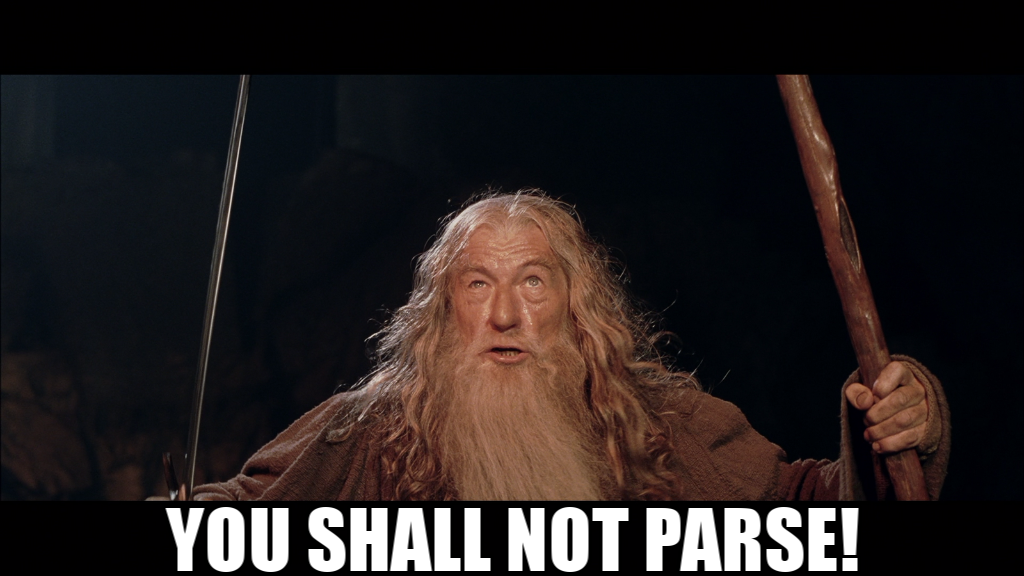
\includegraphics[width=\paperwidth,height=\paperheight]{no-analysis.png}}
	\begin{frame}{Focus on Generation, Ignore Analysis}
	\end{frame}
	}

  \begin{frame}[fragile=singleslide]{Generation: monadic interface}
	We provide a simple monadic interface to allow users to steer the generation process

    \begin{minted}[baselinestretch=1, fontsize=\small, autogobble]{haskell}
type MusicGenerator s a = GenericMusicGenerator GenState s a

type GenericMusicGenerator st s a = StateT (st s) IO a
    \end{minted}
	\end{frame}

    \begin{frame}[fragile=singleslide]{Generation: monadic interface}
	The \icode{GenState} type can be used to generate for the \icode{MusicCore} data type.

    \begin{minted}[baselinestretch=1, fontsize=\small, autogobble]{haskell}
data Entry s a = Entry { values      :: [(Weight, a)]
                       , constraints :: [Constraint a]
                       , selector    :: Selector s a
                       }

data GenState s = GenState { state     :: s
                           , pc    :: Entry s PitchClass
                           , oct   :: Entry s Octave
                           , dur   :: Entry s Duration
                           , itv   :: Entry s Interval
                           , dyn   :: Entry s Dynamic
                           , art   :: Entry s Articulation
                           }
    \end{minted}
	\end{frame}

    \begin{frame}[fragile=singleslide]{Generation: monadic interface}
	\icode{Selector} determines how values are selected from the possible options and \icode{Accessor} tells you how to get to a value in the generation state.

    \begin{minted}[baselinestretch=1, fontsize=\small, autogobble]{haskell}
type Selector s a = s -> [(Weight, a)] -> IO (a, s)

data Accessor st s a = Accessor
  { getValue :: st s -> Entry s a
  , setValue :: Entry s a -> st s -> st s
  }
    \end{minted}

    Default accessors are included for \icode{MusicCore}: \icode{octave}, \icode{duration}, etc ...
	\end{frame}

    \begin{frame}[fragile=singleslide]{Generation: monadic interface}
	Generate a few pitches within the E phrygian dominant scale:

    \begin{minted}[baselinestretch=1, fontsize=\small, autogobble]{haskell}
gen :: MusicGenerator () [PitchClass]
gen = do
  pitchClass >! (inScale E (harmonicMinor ~> P5)
  20 .#. (pitchClass??)
    \end{minted}

    Running the generator (in the IO monad):

    \begin{minted}[baselinestretch=1, fontsize=\small, autogobble]{haskell}
notes <- runGenerator () gen
    \end{minted}
	\end{frame}

    \begin{frame}[fragile=singleslide]{Generation: diatonic improvisation}
	So, how do we go about generating some actual music?
	\end{frame}

    \begin{frame}[fragile=singleslide]{Generation: diatonic improvisation}
	Generating something playable (attempt 1):

    \begin{minted}[baselinestretch=1, fontsize=\small, autogobble]{haskell}
playable = do
  pitches   <- 20 .#. (pitchClass??)
  durations <- 20 .#. (duration??)
  octaves   <- 20 .#. (octave??)
  return (line $ zipWith (<|)
    ((flip (<:) $ []) <$> zipWith (#) pitches octaves)
    durations)
    \end{minted}

    Depending on your taste, this will probably sound rubbish
	\end{frame}

    \begin{frame}[fragile=singleslide]{Generation: diatonic improvisation}
	Generating something playable (attempt 2):

    \begin{minted}[baselinestretch=1, fontsize=\small, autogobble]{haskell}
playable = do
  pitchClass >! (inScale C major)
  options <- (pitchClass?+)
  rhythm  <- boundedRhythm (1 * wn) High
  -- set options and generate pitches
  pitchClass >+ map
        (\(w, v) ->
          if v `elem` (G =| d7 :: [PitchClass])
            then (4 * w, v) else (w, v)) options
  pitches <- (length rhythm) .#. (pitchClass??)
  -- put everything together into a piece of music
  let fullPitches = (flip (<:) $ []) <$>
        (zipWith (#) pitches (repeat 4))
  let gmaj7 = (toMusicCore . chord .
        map (Note (1 * wn) . (flip (#)) 3)) (G =| d7)
  return $ gmaj7 :=: line (zipWith (<|) fullPitches rhythm)
    \end{minted}
	\end{frame}

    \begin{frame}[fragile=singleslide]{Generation: diatonic improvisation}
    Using a simple heuristic and some tweaking, we can improve upon this result:
    \begin{minted}[baselinestretch=1, fontsize=\small, autogobble]{haskell}
diatonicPhrase dur density key scale chord octD = do
    durations <- boundedRhythm dur density
    octaves <- genAspect octave 4
      (length durations) 2.0
        (map (Arrow.first fromIntegral) octD)
    pitches <- genAspect pitchClass key
      (length durations) 1.3
      (mergeWeights
        (intervalWeights key  scale)
        (semiChordWeights key chord))
    let fullPitches = ((flip (<:) $ [])
          <$> (zipWith (#) pitches octaves))
    return $ line
      (zipWith (<|) fullPitches durations)
    \end{minted}
	\end{frame}

    \begin{frame}[fragile=singleslide]{Generation: diatonic improvisation}
    However, as it turns out, this approach doesn't scale too well

    Music is structured in many different ways; both on the micro and macro level.

    The \icode{MusicGenerator} type simply doesn't allow you to generate macro-level structures
    for your music in a nice way. It is too focused on the fundamentals.
	\end{frame}

        \begin{frame}{Chaos in music}
                    \begin{itemize}
                    \item Chaos system: n start values, n update functions. $f_x$ calculates $x_{i+1}$ given $x_{i}$.
                    \item Chaos: small difference in init values gives very different results.
                    \end{itemize}
        \end{frame}
                  
               \begin{frame}{Chaos in music: example}
          \begin{table}[]
                              \centering
                        \caption{$f_x = max\ (-1)\ (min\ 1\ (1 - rx^2))$}
                              \label{my-label}
                              \begin{tabular}{l | lll} % The second | is not an l (L) but a vertical bar!
                              \textbf{r} & \textbf{1.9521} & \textbf{1.9621} & \textbf{0.25} \\
                              \textbf{x} & \textbf{1.2}    & \textbf{1.18}   & \textbf{1.18} \\
                              \hline
                              $x_0$      & -1.0            & -1.0            & 0.8937        \\
                              $x_1$      & -0.9521         & -0.9621         & 0.8002        \\
                              $x_2$      & -0.7695         & -0.8161         & 0.8398        \\
                              $x_3$      & -0.1561         & -0.3070         & 0.8236        \\
                              $x_4$      & 0.9524          & 0.8149          & 0.8304        \\
                              $x_5$      & -0.7708         & -0.3031         & 0.8276        \\
                              $x_6$      & -0.1598         & 0.8196          & 0.8287       
                              \end{tabular}
                      \end{table}
        \end{frame}
        
        \begin{frame}{Chaos in music: hard to get right}
                  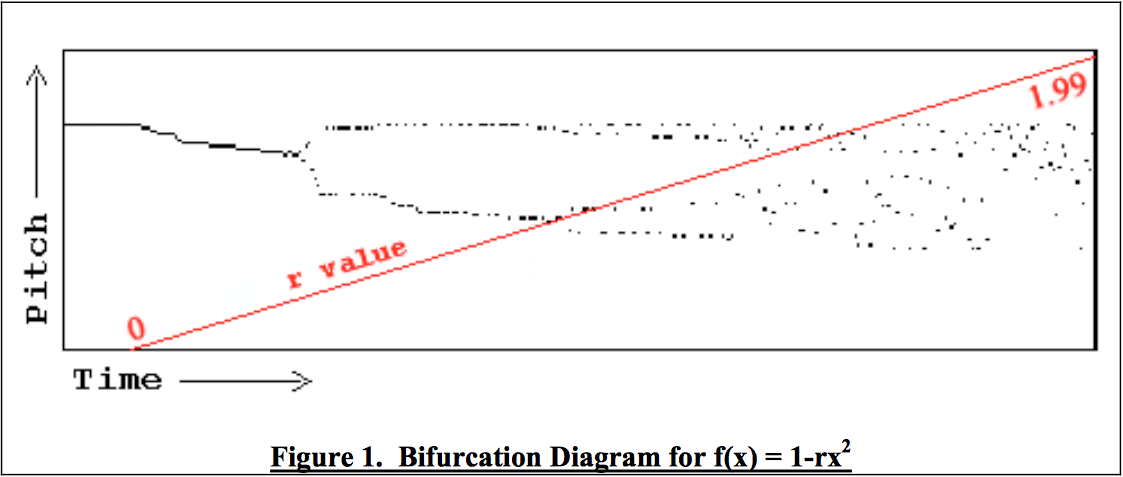
\includegraphics[width=1\textwidth]{figures/chaos.png}\\
                  Walker, Elaine. "Chaos melody theory." Music Technology New York University, Master's thesis (2001).
        \end{frame}

        \begin{frame}{Dynamic Performance: 1 (Cluster notes)}
                    K-means
                    \begin{itemize}
                    \item x: absolute start time of note
                    \item y: pitch, represented as integer
                    \item k: total music time / beats per standard bar
                    \end{itemize}
        \end{frame}
        
        \begin{frame}{Dynamic Performance: 2 (Map to dynamics)}
                    \begin{enumerate}
                    \item	Convert x (abs. time) and y (int pitch) to relative values per cluster in range [0,1].
                    \item Call mapping function on every (x,y) pair
                    \item Convert mapping function result to dynamics
                    \item Add dynamics to note that (x,y) belongs to.
                    \end{enumerate}
        \end{frame}


	\begin{frame}[fragile=singleslide]{Grammars: Properties}
    (Generative) \textit{context-free grammars}, with a few extra features:
	\begin{itemize}
	\item \textbf{Temporal}: Rules are parametric to duration
	\item \textbf{Probabilistic}: Rules can be assigned weights
	\item \textbf{Graph}: Allow node sharing (using \textit{let}-expressions)
	\end{itemize}
	\end{frame}
	
	\begin{frame}[fragile=singleslide]{Grammars: Definition}
	\begin{minted}[baselinestretch=1, fontsize=\small, autogobble]{haskell}
data Grammar meta a =
    a |: [Rule meta a]
data Rule meta a =
    (a, Weight, Dur -> Bool) :-> (Dur -> Term meta a)
data Term meta a =
    a :%: Dur
    | Term meta a :-: Term meta a
    | Aux Bool meta (Term meta a)
    | Let (Term meta a) (Term meta a -> Term meta a)

(a, w) -| f = (a, w, f) :-> (a :%:)
a |->  b = a :-> const b
a |--> b = (a, 1, always) |-> b
($:)  = Aux False
(|$:) = Aux True
	\end{minted}
	\end{frame}
	
	\begin{frame}[fragile=singleslide]{Grammars: Generation}

    	\begin{minted}[baselinestretch=1, fontsize=\footnotesize, autogobble]{haskell}
gen :: (Eq a, Eq meta, Expand input meta a b)
    => Grammar meta a -> input -> Dur -> Music b
gen gr i t = rewrite gr t >>> unlet >>> expand i >>> toMusic
	\end{minted}


	\begin{enumerate}	
	
	\item \textbf{Given an initial duration, rewrite until fixpoint}
	\begin{minted}[baselinestretch=1, fontsize=\footnotesize, autogobble]{haskell}
rewrite :: (Eq a, Eq meta)
        => Grammar meta a -> Dur -> Term meta a
	\end{minted}
	
	\item \textbf{Unfold \textit{let}-expressions}
	\begin{minted}[baselinestretch=1, fontsize=\footnotesize, autogobble]{haskell}
unlet (Let x f) = f x
unlet x         = x
	\end{minted}
	
	\item \textbf{Expand auxiliary wrappers}
	\begin{minted}[baselinestretch=1, fontsize=\footnotesize, autogobble]{haskell}
class Expand input meta a b | input meta a -> b where
    expand :: input -> Term meta a -> Term () b
	\end{minted}
	
	\item \textbf{Convert to music}
	\begin{minted}[baselinestretch=1, fontsize=\footnotesize, autogobble]{haskell}
(:%:) ~> (<|)
(:-:) ~> (:+:)
	\end{minted}
		
	\end{enumerate}
	\end{frame}	
	
	\begin{frame}[fragile=singleslide]{Grammars: Tabla Rhythm}
	\begin{minted}[baselinestretch=1, fontsize=\small, autogobble]{haskell}
tabla :: Grammar () Syllable
tabla = S |:
  [ S  |--> TE1 :-: XI
  , XI |--> TA7 :-: XD
  , XD |--> TA8
  , XG |--> TB2 :-: XA
    ...
  , TE4 |--> Ti :-: Rest :-: Dha :-: Ti
  , TC2 |--> Tira :-: Kita
  , TB3 |--> Dha :-: Tira :-: Kita
  , TD1 |--> Rest
    ...
  ]
instance ToMusicCore Syllable where
    ...
	\end{minted}
	\end{frame}
	
	\begin{frame}[fragile=singleslide]{Grammars: Tonal Harmony}
	\begin{minted}[baselinestretch=0.8, fontsize=\footnotesize, autogobble]{haskell}
harmony :: Grammar Modulation Degree
harmony = I |:
  [ -- Turn-arounds
    (I,  8, (> wn)) :-> \t ->
      Let (I:%:t/2) (\x -> x :-: x)
  , (I,  6, (> hn) /\ (<= wn)) :-> \t ->
      II:%:t/4 :-: V:%:t/4 :-: I:%:t/2
  , (I,  2, (> hn) /\ (<= wn)) :-> \t ->
      V:%:t/2 :-: I:%:t/2
  , (I,  2) -| (<= wn)
    ...
    -- Modulations
  , (V,  5, (> hn)) :-> \t -> Modulation P5 $: I:%:t
  , (V,  3) -| always
  , (II, 2, (> hn)) :-> \t -> Modulation M2 |$: I:%:t
  , (II, 8) -| always
    ...
  ]

instance Expand Config Degree Modulation SemiChord where
    ...

voiceLead :: Music SemiChord -> IO (Music Chord)
	\end{minted}
	\end{frame}	
	
	\begin{frame}[fragile=singleslide]{Grammars: Jazz Improvisation}
	\begin{minted}[baselinestretch=0.8, fontsize=\footnotesize, autogobble]{haskell}
melody :: Grammar () NT
melody = MQ |:
  [ -- Abstract Rhythm { MQ ~> Q }
    (MQ,  1, (== qn)) |-> Q:%:qn
  , (MQ, 25, (> (hn^.))) :-> \t -> Q:%:hn :-: MQ:%:(t - hn)
    ...
    -- Concrete Rhythm { Q ~> MN }
  , (Q, 47, (== wn)) |-> MN:%:qn :-: Q:%:hn :-: MN:%:qn
  , (Q,  6, (== hn)) |->
      MN:%:(qn^^^) :-: MN:%:(qn^^^) :-: MN:%:(qn^^^)
    ...
    -- Abstract Melody { MN ~> N }
  , (MN, 1, (== wn)) |-> N:%:qn :-: N:%:qn :-: MN:%:hn
  , (MN, 1, (== qn)) |->
      N:%:(en^^^) :-: N:%:(en^^^) :-: N:%:(en^^^)
    ...
    -- Concrete Melody { N ~> NT }
  , (N, 50, (== qn)) |-> ChordTone:%:qn
  , (N, 45, (== qn)) |-> Rest:%:qn
  , (N,  1, (== en)) |-> ApproachTone:%:en
    ...
  ]

mkSolo :: Music SemiChord -> Music NT -> IO Melody
    \end{minted}
	\end{frame}
	
	\begin{frame}[fragile=singleslide]{Demo: Code}
	\begin{minted}[baselinestretch=0.9, fontsize=\footnotesize, autogobble]{haskell}
    orientalAlgebras = do
      let ?config = MusicConfig
        { basePc      = A
        , baseOct     = Oct3
        , baseScale   = arabian
        , chords      = equally allChords
        , scales      = equally allScales
        , octaves     = [(20, Oct4), (15, Oct5), (5, Oct6)]
        , restWeight  = 0, ...
        , tempo       = 6%5
        , instruments = [Piano, Sitar, Tabla]
        , beat = sn
        }
      let t = 12 * wn
      har <- voiceLead  <$> runGrammar harmony t
      mel <- mkSolo har <$> runGrammar melody  t
      rhy <- runGrammar tabla t
      writeToMidiFile "out.mid" (dyn (har :=: mel :=: rhy))
	\end{minted}
  	\end{frame}

	\begin{frame}[c]{Demo: Music score}
	\centering
	\vspace{-1.2cm}
	\begin{center}
      \makebox[\textwidth]{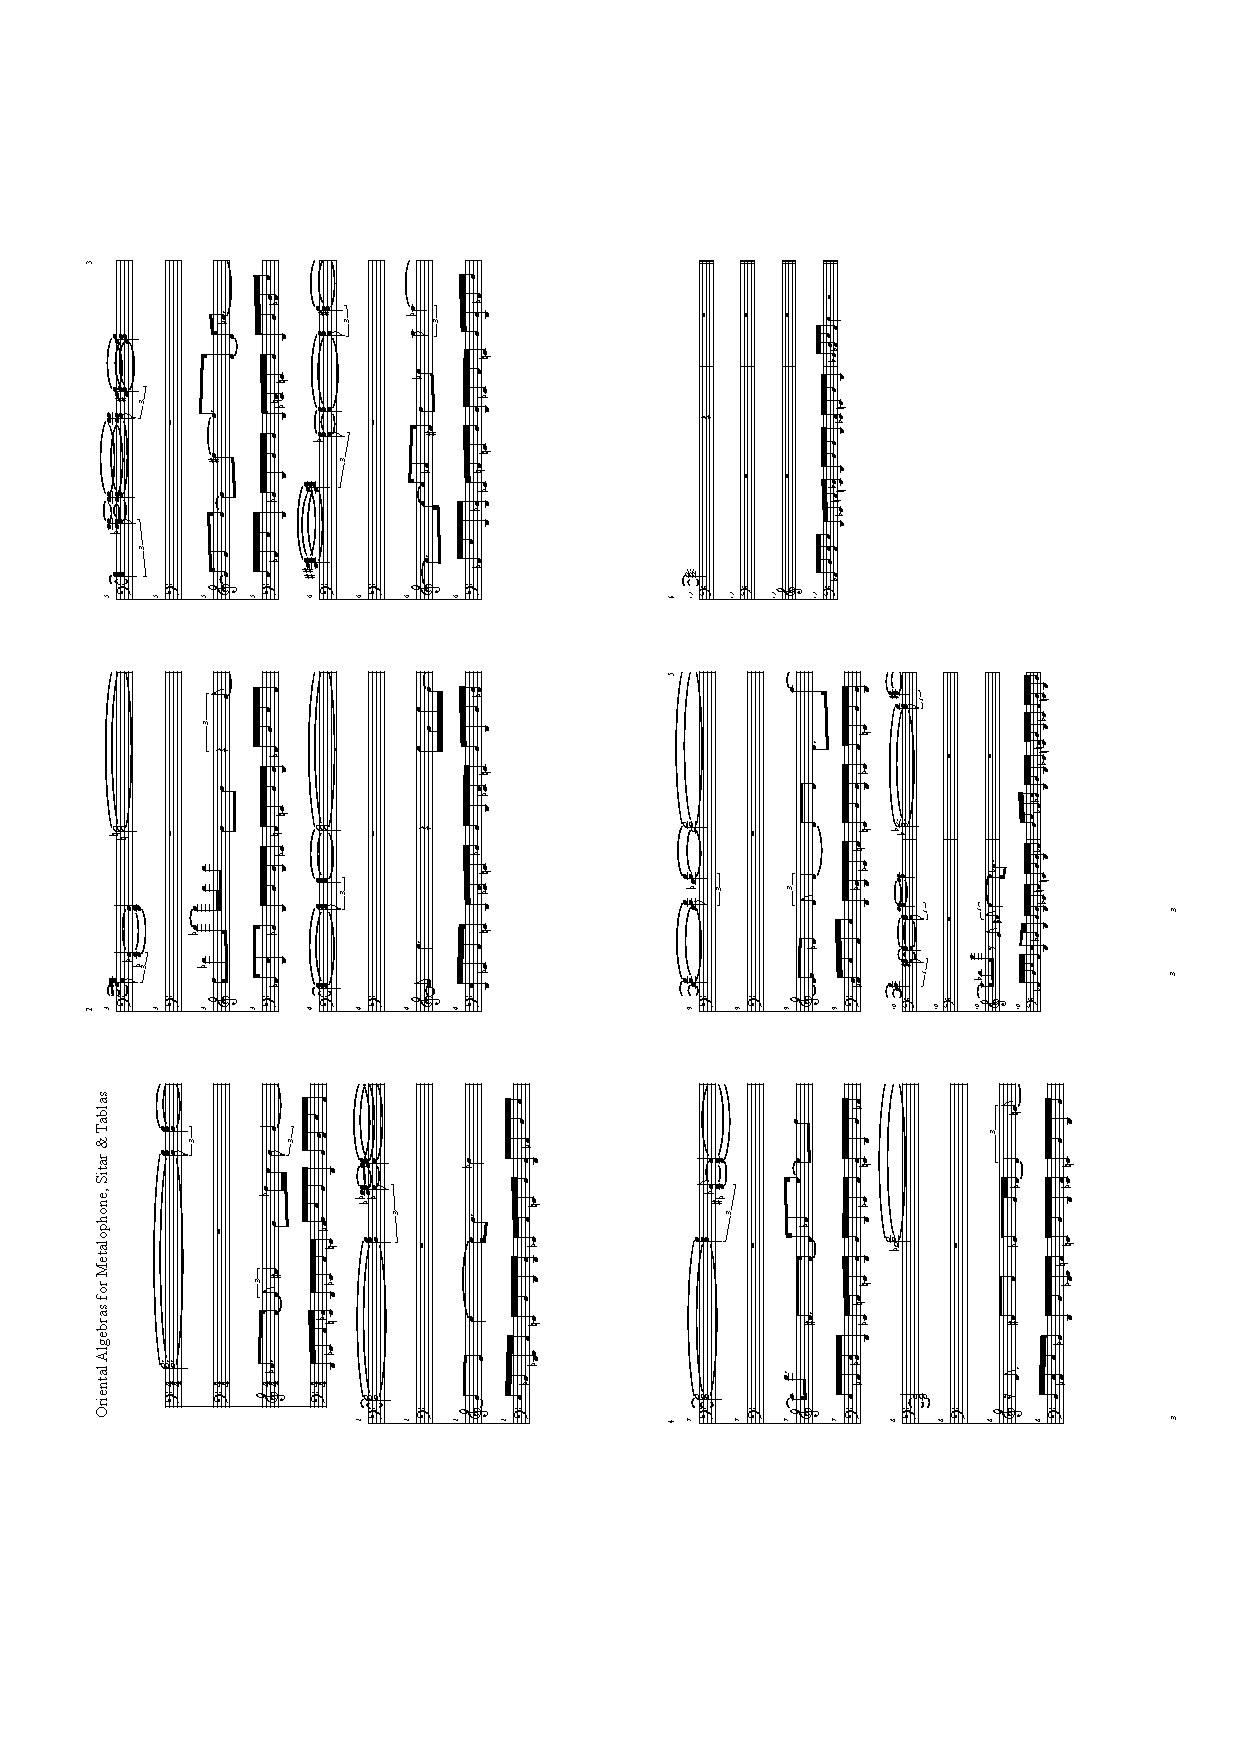
\includegraphics[width=.73\paperwidth,angle=-90]{oriental.pdf}}
    \end{center}
	\end{frame}
  	
\end{document}